% PRAM mit p Prozessoren
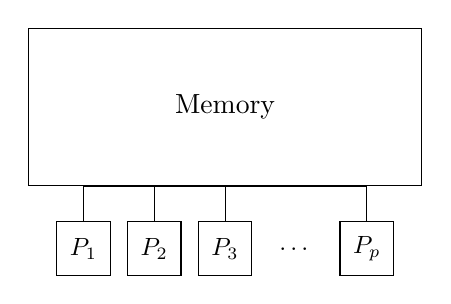
\begin{tikzpicture}
    [
        processor/.style={rectangle, draw, scale=0.9, minimum size=5ex},
        dots/.style={rectangle, scale=0.9, minimum size=5ex},
        scale=0.9,
    ]
    \node (mem) at (3, 2) [
        rectangle,
        minimum height=2cm,
        minimum width=5cm,
        draw,
    ] {Memory};

    \node (p1) at (1,0) [processor] {$P_1$};
    \node (p2) at (2,0) [processor] {$P_2$};
    \node (p3) at (3,0) [processor] {$P_3$};
    \node (p4) at (4,0) [dots] {\ldots};
    \node (pp) at (5,0) [processor] {$P_p$};
    \draw (p1) |- (mem.south);
    \draw (p2) |- (mem.south);
    \draw (p3) |- (mem.south);
    \draw (pp) |- (mem.south);
\end{tikzpicture}         
